\section{Solution}
For our demonstration, we assume that student modelling happens through the use of Bayesian Knowledge Tracing~(BKT)~\cite{bulut2023introduction} which is a common approach in the design of Intelligent Tutoring Systems. However, note that with some modifications, other approaches could also be supported. BKT is a probabilistic model that requires four parameters to be fitted for each learning object as illustrated in \figurename~\ref{fig:bkt}. 
\begin{itemize}
    \item \textbf{$P(L_t)$}: The probability that the topic being covered by the learning object is mastered at time $t$. A value $P(L_0)$ has to be provided to indicate the chance the user knows the topic before attempting any exercise. Note that the topics are defined as a combination of the knowledge topic and the difficulty level as defined later in Section~\ref{subsec:exercises}.
    \item \textbf{$P(S)$}: The probability that the user makes a \emph{slip}, i.e. gets it wrong even though they know the topic.
    \item \textbf{$P(G)$}: The probability that the user makes a lucky guess and gets the answer right even though they do not know the topic.
    \item \textbf{$P(T)$}: The probability that the user actually learns the topic while performing this exercise.
\end{itemize}

\begin{figure}[htb]
    \centering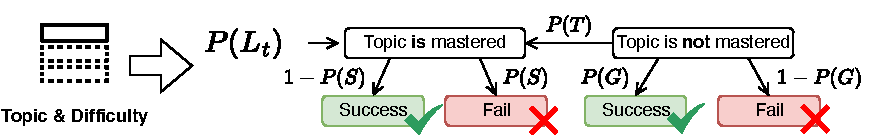
\includegraphics[scale=0.95]{images/BKT.pdf}
    \caption{Example of the Bayesian Knowledge Tracing model per topic and difficulty pair}\label{fig:bkt}
\end{figure}

Based on these values, we can then calculate the updated probability that a topic (e.g.~``Arrays") is mastered each time the user is presented with a new exercise about this topic ($L_{t+1}$) based on whether they succeeded or failed solving the exercise. It is important to note that all these probabilities are exercise dependent and will as such not be shared across the applications except for $P(L_t)$. This value is the probability that the user knows a topic, which can be shared across any application as long as they are referring to the same topic.  

We aim to store the result of every exercise the user performs within a personal data vault, together with the calculated $P(L_t)$ for every topic and difficulty~level pair as shown in \figurename~\ref{fig:overview}. Developers of educational applications could then request limited-time access to the entries of all of their users in order to fit their models, without the need to permanently own all the data. Shared information, such as the $P(L_t)$, will further make it easier for other developers to contribute their own extensions that provide exercise recommendations.

\begin{figure}[htb]
\begin{minipage}[t]{0.39\textwidth}
\vspace{0pt}
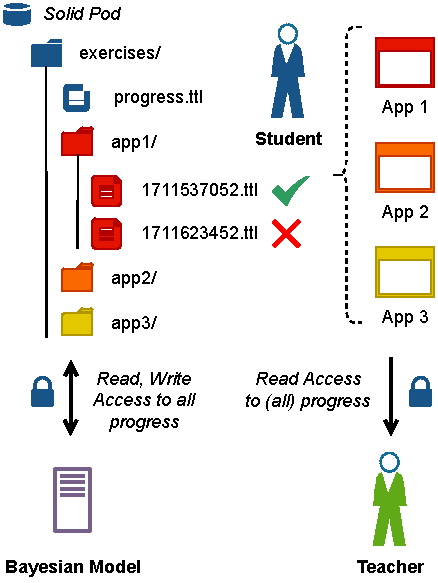
\includegraphics[width=\textwidth]{images/SoSyYoshi.drawio.pdf}
\vspace{0pt}
\caption{Overview of individual apps \\ 
storing exercise results in a Solid Pod}
\label{fig:overview}
\end{minipage}\hfill
\begin{minipage}[t]{0.59\textwidth}
\vspace{0pt}
\begin{minted}[xleftmargin=0pt,fontsize=\small]{turtle}
<> a schema:ReplyAction; # A reply to a question
  dct:created "2024-03-28T11:57"^^xsd:dateTime;
  schema:agent <http://.../profile/card#me>;
  # Exercise question
  schema:parentItem [ a schema:Question;
    schema:name "What is the output of ...?"@en;
    schema:educationalLevel primm:Predict;
    schema:eduQuestionType "Flashcard"@en;
    foaf:topic dbr:Array;
    foaf:agent <https://app1.org/>. # Creator
  ];
  schema:result [ a schema:Answer; # User answer
    schema:answerExplanation [ ... ];
    schema:review [ a schema:Review;
      # The grade of the answer (e.g. 5 out of 5)
      schema:reviewRating 5; schema:bestRating 5.
    ]
  ].
\end{minted}
\vspace{3.6pt}
\captionof{listing}[]{Example reply on a question generated by app \#1\\
using prefixes \texttt{dbr}~\cite{10.1007/978-3-540-76298-0_52}, \texttt{schema}~\cite{10.1002/asi.24744}, \texttt{foaf}~\cite{brickley2007foaf} and \texttt{dct}~\cite{weibel1998dublin}}
\label{lst:exercise}
\end{minipage}
\end{figure}

Users can already indicate their topics of interest in their Solid Pod using the topics of interest predicate from the \texttt{foaf} vocabulary~\cite{brickley2007foaf}, which can aid educational recommendation systems to provide exercises that interest the user. Together with data about the past performance, we can create personalised learning paths for users based on their strengths and weaknesses from multiple sources without creating any vendor lock-in and without claiming ownership of the students' data.

In addition, the progress of these exercises and topics can optionally be shared with an educator or mentor as illustrated in \figurename~\ref{fig:overview}, allowing for personalised feedback and guidance to further support a user's learning journey. The fine-grained control over the data also allows students to share the information on topics they are currently covering in class, while preventing the need to share that they are still working on other topics that they do not want to share.

\subsection{Exercises and Progress} \label{subsec:exercises}
Each topic has a set of exercises with their individual difficulty level. With our proposed solution we use the existing \mbox{PRIMM} principles~\cite{sentance2019teaching} to identify the five stages of difficulties for exercises. These stages include the ability to \textit{predict} the output of a piece of code, \textit{run} a piece of code, \textit{investigate} a piece of code and answer some questions about its structure, \textit{modify} a piece of code so the behaviour changes to a new desired result and finally, \textit{make} a similar piece of code from scratch. Together, these five principles identify the logical progression of difficulty levels with which to look at a piece of code from the perspective of a student. Listing~\ref{lst:exercise} illustrates an example exercise and the answer given to this exercise that includes the difficulty level\footnote{The \texttt{primm:} vocabulary represents a trivial vocabulary to describe the difficulty levels in programming exercises} using the \texttt{educationalLevel} predicate. 

A further extension of the architecture would allow third-party developers to share the capabilities of their plugins with regards to what type of content their plugins could provide so the recommendation engine can be a fully separate component querying all content providers included by the user without it being centrally controlled by one individual.

\begin{listing}[htb]
\begin{minted}[xleftmargin=0pt,fontsize=\small]{turtle}
<#progress_arrays_predict> a sosa:ObservableProperty ;
    rdfs:label "Prediction progress"@en ; ssn:isPropertyOf <#me> ; 
    foaf:topic dbr:Array ; schema:educationalLevel primm:Predict .
<#1711623452> a sosa:Observation ; # P(L_(t+1))
    sosa:usedProcedure dbr:Bayesian_Knowledge_Tracing ;
    dct:created "2024-03-28T11:57"^^xsd:dateTime ;
    foaf:agent <https://app1.org/> ; sosa:observedProperty <#progress_array> ;
    sosa:hasResult [ qudt:floatPercentage "38.12"^^xsd:float ] .
<#1711537052> a sosa:Observation ; # P(L_t)
    sosa:usedProcedure dbr:Bayesian_Knowledge_Tracing ;
    dcterms:created "2024-03-27T11:57"^^xsd:dateTime ;
    foaf:agent <https://app1.org/> ; sosa:observedProperty <#progress_array> ;
    sosa:hasResult [ qudt:floatPercentage "25.0"^^xsd:float ] .
\end{minted}
\vspace{-4pt}
\centering
\caption{Multiple observations of user progress for a particular topic and difficulty level} \label{lst:progress}
\vspace{-2pt}
\end{listing}

Listing~\ref{lst:progress} shows multiple observations of user progress for a particular topic at a given time (i.e.~$P(L_t)$). Each observation, described using the SOSA ontology~\cite{janowicz2010stimulus,janowicz2019sosa}, is created by an application. This progress is shared, allowing each educational application to use these observations to determine the current knowledge on a topic.


